\documentclass{article}

%\usepackage[
  paperheight=8.5in,
  paperwidth=5.5in,
  left=10mm,
  right=10mm,
  top=20mm,
  bottom=20mm]{geometry}
\usepackage[utf8]{inputenc}

%%\usepackage{biblatex}
\usepackage{graphicx}
\usepackage{wrapfig}
\usepackage[bottom]{footmisc}
\usepackage{listings}
\usepackage{enumitem}

\usepackage{wrapfig}
\usepackage{ragged2e}

\usepackage{array}
\usepackage[table]{xcolor}
\usepackage{multirow}
\usepackage{booktabs}
\usepackage{hhline}
\definecolor{palegreen}{rgb}{0.6,0.98,0.6}

\usepackage{amsmath}
\usepackage{amssymb}
\usepackage{multicol}
\usepackage{lipsum}
\usepackage{hyphenat}
\PassOptionsToPackage{hyphens}{url}
\usepackage{url}

\usepackage{rotating}

\usepackage{pdfpages}

%% support use of straight quotes in code listings
\usepackage[T1]{fontenc}
\usepackage{textcomp}
\usepackage{listings}
\lstset{upquote=true}

%% for shrinking space between lines
\usepackage{setspace}

\usepackage{caption}

\newcommand*{\affaddr}[1]{#1} % No op here. Customize it for different styles.
\newcommand*{\affmark}[1][*]{\textsuperscript{#1}}
\newcommand*{\email}[1]{\small{\texttt{#1}}}
\newcommand{\tarot}{\textsc{Tarot}}
\renewcommand*\contentsname{\centering Table of Contents}

\renewcommand{\footnoterule}{%
  \kern -3pt
  \hrule width \textwidth height 0.5pt
  \kern 2pt
}

\usepackage{titlesec}
\titleformat*{\section}{\large\bfseries}
\titleformat*{\subsection}{\normalize\bfseries}
\titleformat*{\subsubsection}{\normalize\bfseries}

% define variables
\newcommand{\confOrdinal}{34th}
\newcommand{\confName}{South Central}
\newcommand{\confDates}{March 31st}
\newcommand{\confYear}{2023}
\newcommand{\confSchool}{Stephen F. Austin State University}
\newcommand{\confCity}{Nacogdoches, TX}
\newcommand{\journalVolume}{38}
\newcommand{\journalNumber}{7}
\newcommand{\journalMonth}{April}
\newcommand{\journalYear}{2023}
\newcommand{\regionalEditor}{Mustafa Al-Lail}
\newcommand{\regionalEditorSchool}{Texas A\&M International University}



%%\addbibresource{sample.bib}

\title{Iterative Efforts for Improving Learning Experience in Software Engineering\footnote{\protectCopyright \copyright \confYear\ by the Consortium for Computing Sciences in Colleges.
Permission to copy without fee all or part of this material is granted provided
that the copies are not made or distributed for direct commercial advantage,
the CCSC copyright notice and the title of the publication and its date appear,
and notice is given that copying is by permission of the Consortium for
Computing Sciences in Colleges.  To copy otherwise, or to republish, requires
a fee and/or specific permission.
}
}



\author{
Pradip Peter Dey, Mohammad Amin and Bhaskar Raj Sinha\\
School of Technology and Engineering\\
National University\\
9388 Lightwave Ave., San Diego, CA 92123\\
\email{\{pdey, mamin, bsinha\}@nu.edu}\\
}

\begin{document}
\maketitle

\begin{abstract}
In a project-based learning environment, students and teachers jointly made iterative efforts for improving learning experience in software engineering through all major tasks including requirements analysis, design, implementation, and testing. The iterative efforts were implemented in a prototype-based evolutionary process 
by performing reviews jointly by students and teachers after each major task, and assessing student performance based on their participation in task-related activities. End of course evaluation data, collected in a standard anonymous process, indicated improvements in student learning experience and teaching effectiveness attributable to the iterative efforts. The major advantages of the iterative efforts were 
engaging students in the review process, and eliminating or reducing plagiarism-based academic dishonesty by emphasizing participation-based grading. One of the major challenges for teachers was making extra efforts for participation-based grading, rather than using automated grading of multiple choice exams and quizzes.  In 
addition, extra efforts were needed to complete three iterations for sizable software engineering projects in a timely manner in order get benefits of iterative efforts in project-based learning environments. There are opportunities for future research in this area for creating a set of revealing software engineering projects of appropriate sizes and explaining their potential benefits in teaching learning environments.   

\end{abstract}

\section{Introduction}
In a project-based learning environment \cite{guo}, teachers and students can work together cooperatively performing software requirements engineering, design, implementation and testing, and their reviews iteratively in 
order to promote desirable learning 
experience \cite{sokhan} and 
fair grading.  
Key development skills are in demand because developers are facing increasingly more complex problems in their work environment. Design skills are more important than other skills, because ``The ability to recognize complexity is a crucial design skill'' \cite{ouster} (page 5). When a designer recognizes that a system is too complicated, the designer can use that ability to guide their design philosophy towards dealing with the complexity \cite{ouster}.  Designers should be able to explain how the software elements will work together collaboratively in operational scenarios to provide appropriate services to users with excellent user experience. 

Great designers such as Steve Jobs and Jony Ive (of Apple, Inc.) have not described their innovative design approaches for teaching-learning purposes \cite{isaacson}.  Jason Hong has studied the practices in Apple, and asked the following question ``Why is great design so hard?'' \cite{hong}. In this paper, we critically examine some teaching strategies for making iterative efforts for improving learning experience in design, and suggest that one of the strategies has great potential in project-based learning \cite{guo}. For explaining the potential, we emphasize graphical user interface (GUI) design. Evidence from end of course evaluation data, collected in a standard anonymous process, is presented that indicates improvements in students learning experience and teaching effectiveness attributable to iterative efforts.

\section{Iterative Efforts}
Iterative efforts for software engineering can be made with well-known process models such as evolutionary, spiral, agile, or prototype-based development 
models \cite{braude, giacomin, kung, ouster, pfleeger, pressman, rumbaugh, shneiderman, sommerville}. Iterative efforts using evolutionary prototypes are often recommended in object oriented software development \cite{kung, rumbaugh}.  One can follow Pressman and Maxim’s textbook which suggests that ``Software design is an iterative process . . .'' \cite{pressman} (page 228).  Designers can make excellent progress through successive refinement in 
an iterative process. Most process models allow design reviewers and designers to ask questions such as, ``Is this the best possible design for this product? Or, are there opportunities for improvement?''  Iterative efforts with these types of questions promote innovations as demonstrated by Steve Jobs and Jony Ive \cite{isaacson}.  Effective GUI designers repeatedly examine their designs in order to make improvements where many alternatives are carefully considered. GUI design and development cannot be done in a hurry considering only some obvious alternatives.  Experiments with evolutionary prototypes and their careful reviews may focus on providing excellent user 
experience \cite{kung, pressman}.

\section{Reviews in Software Engineering}
All major tasks in software engineering should be reviewed for preventing errors or defects.   Software requirements engineering, design, implementation, testing and their reviews may be introduced to students using examples and textbooks \cite{kung, pressman}.  A good strategy for initial design is to decompose the problem into several sub-problems or relatively independent conceptual elements \cite{ouster}. However, this strategy requires some understanding of interactions among the conceptual elements. Use cases and their relationship from requirements engineering may help at this stage \cite{pressman, rumbaugh}. Following the Unified Modelling Language (UML), one can also draw use case diagrams \cite{pressman, rumbaugh}.  Preliminary reviews can start with the use case diagrams.  For better reviews, other UML diagrams including component diagram, class diagram, sequence diagram, state machine diagram, and activity diagram may be considered \cite{pressman, rumbaugh}. A use case diagram presents major use cases with ovals in a box or rectangle displaying actors outside the box to indicate that the actors are external users of the current system. Each use case represents a case of use that can be further illustrated in other UML diagrams such as activity diagrams, sequence diagrams \cite{pressman, rumbaugh}.  Consider a sample use case diagram shown in Figure 1; it was drawn in the UML 2.0 notation with a minor extension for a sample software project, which was initially described as follows:  

 \emph{``Develop a software system for computing areas of three types of play-place units: Rectangular, Circular and Triangular. A contractor in Los Angeles builds play-places (with materials such as wood, iron, pads, plastics etc.) at customer site using play place units of different dimensions. The charges are in dollars based on the area of each unit 
in square feet, plus the number of units. The software system is needed for computing the cost which is based on area. 
The cost is five dollars per square foot. Assume that users always use feet for entering the dimensions of the units. A Graphical User Interface (GUI) is required for user interactions. Additional typical assumptions can be made about this project.''} 

In addition to the above sample problem, Albrecht’s function point method \cite{albrecht} was used for explaining iterative efforts (a prototype for function point estimation is available at http://www.asethome.org/project/functionpoint.html). Iterative efforts for major tasks and their reviews were explained with two textbooks \cite{kung, pressman}.  The interfaces shown with the dotted rounded rectangles in Figure 1 were explained with special care, because these were absent in the standard UML use case diagrams \cite{pressman, rumbaugh}. These dotted interfaces were called general interfaces in order to distinguish them from specialized UML interfaces such as provided interfaces and required interfaces [14]. In order to conveniently refer to the general interfaces, they were sequentially numbered. A general interface shown within the system box must be developed as a part of the current software system; otherwise, it should be depicted outside the system boundary (such an interface is usually available in the development environment). If an interface was a GUI, then it was marked with the term “GUI” utilizing UML stereotypes \cite{rumbaugh}.   

It was reasonable to be flexible about the notations of the diagrams, because we needed to emphasize design skills, and not necessarily the diagram notations. Practitioners in agile development techniques value ``Working software over comprehensive documentation" \cite{beck}.  Following the “Manifesto for Agile Software Development”, we emphasized working software that may satisfy end-users in operational 
environments \cite{beck}. In our project-based environment, the primary measure of progress in software development was working software, not extensive documentation with precise diagrams in standard notations. We considered two main alternative notations for the general interface diagrams: (1) screen shots from a prototype, and (2) abstract graphical representation of major interface elements. We show the former notation in the general interface diagram given in Figure 2 for the general interface 1 of Figure 1.  The GUI in Figure 2 is from our third iteration.   


\begin{figure}
    
 \centering
    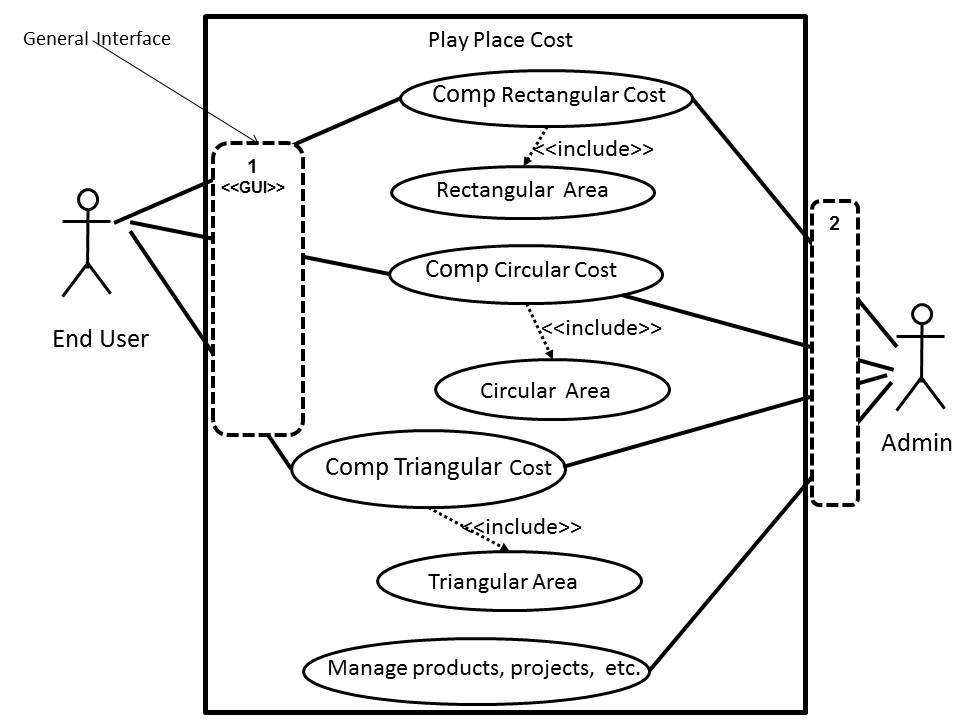
\includegraphics[width=0.9\textwidth]{191_1.jpg}
  \caption{\label{fig:UseCasePlayPlace}Augmented use case diagram with general interfaces.}
 

\end{figure} 


\begin{figure}
    
 \centering
    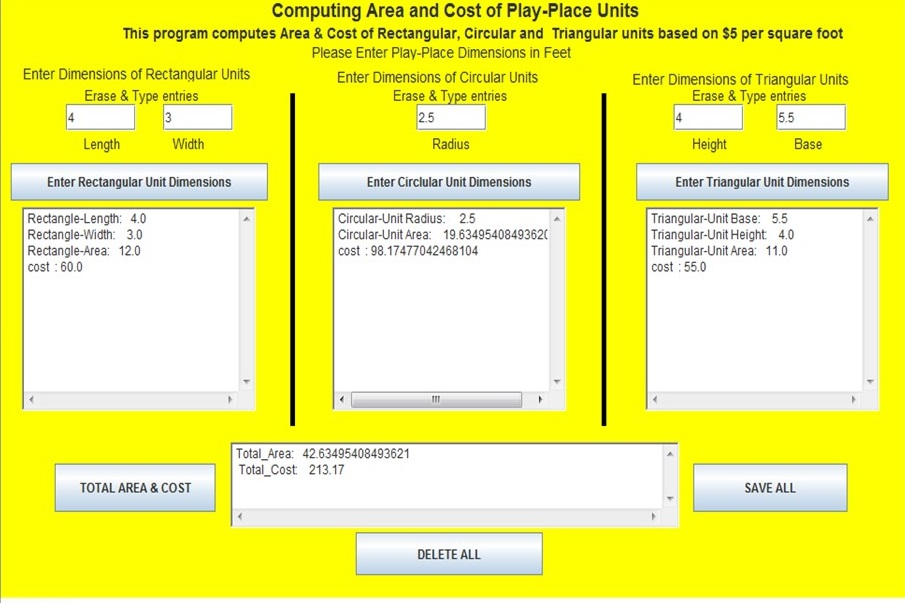
\includegraphics[width=0.9\textwidth]{191_2.jpg}
   \caption{\label{fig:_GUIplayPlace}A prototypical general interface diagram (from third iteration)}

\end{figure} 

\section{Guidelines for Design}
As designers and design-reviewers go through the iterative process they may like to follow some guidelines. Most of the guidelines suggested below came from Pressman and Maxim \cite{pressman}; others were inspired by Hong \cite{hong}, and Kung \cite{kung}.       



\begin{enumerate}
  \item Examine promising alternatives from the widest range of possible alternatives in order to provide the best user experience through integration of various features including artistic, mathematical and intuitive aspects.
  \item Utilize Object Oriented Design concepts throughout the development process.  
  \item Consider separation of concerns in order to deal with complexity of the system and interactions among system elements.
  \item Consider design principles as well as human-computer interaction (HCI) data and user experience for innovative user interface solutions. 
  \item Include only those action features which are intuitively learnable; transform others to an automated category.
  \item Maximize cohesion and minimize coupling among components.
  \item Include error prevention and simple error handling.
  \item Present design models at multiple levels of abstraction. 
  \item Make iterative efforts through design-review-redesign as many times as possible using the guidelines 1 through 8.
\end{enumerate}

With reference to guideline 1, innovative designers often consider many unusual alternatives in addition to obvious ones. Quick design in a hurry may lead to consideration of only a few obvious alternatives missing innovative solutions \cite{hong, isaacson}. Steve Jobs and Jony Ive came up with brilliant user interface solutions that were missed by other practitioners in the same 
domain \cite{hong, isaacson}. Object-oriented design of guideline 2 is emphasized in several popular books \cite{kung, pressman}.  Object-oriented design elements such as fields, windows, buttons, allow rapid prototyping \cite{kung, pressman}. Guideline 3 is essential for solving complicated problems \cite{ouster, pressman}.  Guideline 4 is based on a reasonable integration of HCI factors \cite{shneiderman}, user experience, and other advanced design strategies \cite{pressman, rumbaugh, shneiderman}. Guideline 5 suggests that users should not be burdened by cognitive load and difficult learning tasks \cite{pressman, shneiderman}. If there are tasks that are not easy to learn, the designer should try to automate them as much as possible. Guideline 6 is suggested in many popular 
books \cite{kung, pressman}. Guideline 7 is important for dealing with errors \cite{braude, kung, ouster, pfleeger, pressman, rumbaugh, shneiderman, sommerville}; it is related to guidelines 3 and 6 because loosely coupled systems have advantages over tightly coupled systems. It is easy to make changes to loosely coupled components. Guideline 8 makes sure that the design is expressible in multiple levels of abstraction without significant loss of clarity. When one level of abstraction is transformed into another level, consistent interpretations should be
applicable to both levels. Presenting user interface designs in multiple levels may help thorough reviews.  Most designers are inspired by the success of Steve Jobs and Jony Ive’s design \cite{hong, isaacson}.  Steve Jobs and Jony Ive were committed to Apple’s proclamations such as “Simplicity is the ultimate sophistication” \cite{isaacson}. They achieved simplicity by conquering complexities, not ignoring them \cite{isaacson}. Jobs and Ive forged a bond that led to “the greatest industrial design collaboration of their era” \cite{isaacson} (page 341).  

Iterative efforts outlined above were implemented in a project-based learning environment \cite{guo} with a special emphasis on design and design review. Students were introduces to the iterative efforts with an example before they began their work on their projects. Students started their project work with requirements engineering and submitted their initial requirements analysis, which was reviewed jointly by teachers and students. In the next step, students designed the system that was followed by a design review jointly by students and teachers, followed by development of version-2 design, which was submitted by the students within a few days; this was followed by version-2 design review (jointly by students and teachers). In the next step an evolutionary prototype was implemented by the students;  this prototype was then reviewed jointly by students and teachers. Based on the review, the system was redesigned again and this new design was reviewed and implemented.  Another iteration of design, design review, implementation and testing was performed.  Evidence from the end of course evaluation indicates that before the iterative efforts method was put into practice, the overall mean students’ self-assessment of learning was 4.78 and the overall mean students’ teaching evaluation was 4.73. After the practice, the learning figure rose to 4.96, and the teaching figure rose to 4.97.  Evaluations by faculty panels suggest that students’ performance had also improved according to outcomes based assessments \cite{guo, sokhan}. Iterative efforts suggested here may provide extra benefits towards fair grading based on students’ participation in the project activities, rather than on written assignments, which can be generated completely or partly by AI tools such as ChatGPT, or other chat-bots \cite{alkhatlan, mollick, welsh}. It is becoming possible for AI tools to generate discussion board posts, write student papers based on a few prompts, and provide answers to essay questions on exams. Unacknowledged use of an AI tool such as ChatGPT to write essays, answer exam questions, write discussion board posts, or to complete many types of assignments may be considered ethically unacceptable. A few reasonable ways to adjust the course contents, delivery methods, and student evaluation in software engineering include project based learning \cite{guo}, evaluation with case studies, iterative hands-on design, design reviews, and other collaborative activities. However, iterative efforts require additional time in order to complete three iterations for sizable projects, because fair assessment necessitates that adequate opportunities must be provided for student participation in all major software engineering activities \cite{guo}.        

\section{Concluding Remarks}
We have examined certain challenges of teaching software engineering and suggested opportunities for improvement based on our experiments with project-based learning \cite{guo}. Iterative efforts may offer opportunities for overcoming some of the challenges. Some extra benefits of teaching iterative efforts include engaging students in the collaborative review of all major software engineering tasks in each iteration, and outcomes based assessment for fair grading. A set of guidelines is evolving from the studies of successful design and development practices; these guidelines have great potential for helping software engineers, and providing clarity about the nature of improvements that are achievable through iterative efforts in software engineering. From practical experience of software engineers, the guidelines can be reviewed and revised.  There are opportunities for future research in this area for creating a set of revealing software engineering projects of appropriate sizes and explaining their potential benefits in project based learning environments.  In addition, future work may include how to deal with ethical concerns about use of smart AI tools in teaching learning environments.    

\medskip

%%\printbibliography
\bibliographystyle{plain}
\bibliography{191}


\end{document}
